%template1.tex
%The following LaTeX source file represents the simplest kind of slide presentation; no overlays, no included graphics. Substitute your favorite style for ``pascal''. To create the PDF file template1.pdf, (1) be sure to use the prosper class, then (2) execute the command latex template1.tex, and (3) the command dvipdf template1.dvi.

%%%%%%%%%%%%%%%%%%%%%%%%%%%%%%% template1.tex %%%%%%%%%%%%%%%%%%%%%%%%%%%%%%%%%%%
\documentclass[a4paper,blends,pdf,colorBG,slideColor]{prosper}
% definitions for slides for CSC544
% Lutz Hamel, (c) 2007

\hypersetup{pdfpagemode=FullScreen}

\usepackage{amssymb}
\usepackage{latexsym}
\usepackage{amsmath}
%\usepackage[usenames]{color}
\usepackage{xypic}


\newcommand{\term}[1]{\ensuremath{\mbox{\bf #1}}}
\newcommand{\nonterm}[1]{\ensuremath{\mbox{#1}}}
\newcommand{\ifstmt}[3]{\ensuremath{{\bf if}\; {#1}\;{\bf then}\;{#2}\;{\bf else}\;{#3}\;\term{end}}}
\newcommand{\whilestmt}[2]{\ensuremath{{\bf while}\; {#1}\;{\bf do}\;{#2}\; \term{end}}}
\newcommand{\funcstmt}[3]{\ensuremath{{\bf fun}\; {#1}\; {\bf is}\; {#2} \; {\bf return}\; {#3}}}
\newcommand{\syntaxset}[1]{\ensuremath{\mbox{\bf #1}}}
\newcommand{\orbar}{\;|\;}
\newcommand{\bs}[1]{\begin{slide}{#1}\ptsize{8}}
\newcommand{\es}{\end{slide}}
\newcommand{\co}{\,\colon\;}
\newcommand{\pair}[2]{\ensuremath{\langle {#1}, {#2} \rangle}}
\newcommand{\encode}[1]{\ensuremath{\langle {#1} \rangle}}
\newcommand{\mytab}{\makebox[.15in]{}}
%\newcommand{\abs}[1]{{\mid{#1}\mid}}
\newcommand{\abs}[1]{{|{#1}|}}
\newcommand{\ol}[1]{\overline{#1}}

\newcommand{\qaccept}{\ensuremath{q_{\mbox{\tiny accept}}}}
\newcommand{\qreject}{\ensuremath{q_{\mbox{\tiny reject}}}}
\newcommand{\accept}{{\em accept}}
\newcommand{\reject}{{\em reject}}

\newcommand{\machine}[1]{
	\begin{quote}
	{#1}
	\end{quote}
	}

\newcommand{\fdef}[1]{
	\begin{center}
	\fbox{
	\begin{minipage}{3.5in}
	{\bf Definition:}
	{#1}
	\end{minipage}
	}
	\end{center}
	}

\newcommand{\ftheorem}[1]{
	\begin{center}
	\fbox{
	\begin{minipage}{3.5in}
	{\bf Theorem:}
	{#1}
	\end{minipage}
	}
	\end{center}
	}

\newcommand{\flemma}[1]{
	\begin{center}
	\fbox{
	\begin{minipage}{3.5in}
	{\bf Lemma:}
	{#1}
	\end{minipage}
	}
	\end{center}
	}


\newcommand{\fframe}[1]{
	\begin{center}
	\fbox{
	\begin{minipage}{3.5in}
	{#1}
	\end{minipage}
	}
	\end{center}
	}

\newcommand{\nframe}[1]{
	\begin{center}
	\begin{minipage}{3.5in}
	{#1}
	\end{minipage}
	\end{center}
	}

\begin{document}

\bs{$\mu$-Recursive Functions}
\small
Here we investigate the relationship between Turing machines and
computable functions.

For convenience we will restrict ourselves to only look at numeric computations, this
does not reflect any loss of generality since all computational problems can be
encoded as numbers (think ASCII code).  Kurt G\"{o}del used this fact in his famous
{\em incompleteness proof}.

We will show that,

\nframe{The functions computable by a Turing machine are exactly the $\mu$-recursive
functions.}

$\mu$-recursive functions were developed by G\"{o}del and Stephen Kleene.  

So, between Turing, Church, G\"{o}del,
and Kleene we obtain the following equivalence relation:


\fframe{
\[\mbox{
Algorithms $\Leftrightarrow$ Turing Machines $\Leftrightarrow$ $\mu$-Recursive Functions $\Leftrightarrow$
$\lambda$-Calculus}
\]} 

In order to work towards a proof of this equivalence we start with {\em primitive recursive functions}.
\es

\bs{Function Composition}
{\small
A more general view of function composition in order to define primitive recursive functions,
\fframe{Let $g_1,g_2,\ldots,g_n$ be $k$-variable functions and let $h$
be an $n$-variable function, then the $k$-variable function $f$ defined by
\[
f(x_1,\ldots,x_k) = h(g_1(x_1,\ldots,x_k),\ldots,g_n(x_1,\ldots,x_k))
\]
is called the {\bf\em composition} of $h$ with $g_1,g_2,\ldots,g_n$ and is 
written as
\[
f = h\circ(g_1,\ldots,g_k).
\]}
{\bf NOTE:} The function $f(x_1,\ldots,x_k) $ is undefined or $f(x_1,\ldots,x_k) \uparrow$ if either
\begin{enumerate}
\item $g_i(x_1,\ldots,x_k)\uparrow$ for some $1\le i \le n$, or
\item $g_i(x_1,\ldots,x_k) = y_i$ for $1\le i \le n$ and $h(y_1,\dots,y_n)\uparrow$.
\end{enumerate}

{\bf NOTE:} Here $g(\cdot)\uparrow$ means that $g$ is undefined.

{\bf NOTE:} Composition is strict in the sense that if any of the arguments of
a function are undefined then so is the whole function.

}
\es

\bs{Function Composition}
A function $f$ is called a {\bf\em total function} if it is completely defined over its domain, that is, $\forall x, f(x)\downarrow$.\footnote{You guessed it, the $\downarrow$ indicates
that the function is defined.}

A function $f$ is called a {\bf\em partial function} if it is undefined for at least one
element in its domain, that is, $\exists x, f(x)\uparrow$.

\vspace{1.5in}

\es


\bs{Primitive Recursive Functions}
{\small
\fdef{The basic {\bf\em primitive recursive functions} are defined as follows:
\begin{description}
\item[zero function:] $z(x) = 0$ is primitive recursive
\item[successor function:] $s(x) = x + 1$ is primitive recursive
\item[projection function:] $p^{(n)}_i(x_1,\ldots,x_n) = x_i, 1 \le i \le n$ is primitive recursive
\end{description}
More complex primitive recursive function can be constructed by a finite number of
applications of,
\begin{description}
\item[composition:] let $g_1,g_2,\ldots,g_n$ be $k$-variable primitive recursive functions and let $h$
be an $n$-variable primitive recursive function, then the $k$-variable function $f$ defined by
\[
f(x_1,\ldots,x_k) = h(g_1(x_1,\ldots,x_k),\ldots,g_n(x_1,\ldots,x_k))
\]
is also primitive recursive.
\item[primitive recursion:] let $g$ and $h$ be primitive recursive functions with $n$ and $n+2$ variables, respectively,
then the $n+1$-variable function $f$ defined by
\begin{enumerate}
\item $f(x_1,\ldots,x_n,{\color{red}0}) = g(x_1,\dots,x_n)$
\item $f(x_1,\ldots,x_n,{\color{red}s(y)}) = h(x_1,\dots,x_n,{\color{red}y},f(x_1,\ldots,x_n,{\color{red}y})$
\end{enumerate}
is also primitive recursive.
Here, the variable $y$ is called the {\bf\em recursive variable}.
\end{description}
}
\begin{center}
{\bf Observation:} The primitive recursive functions are total functions.
\end{center}
}
\es

\bs{Primitive Recursive Functions}
Why are primitive recursive functions interesting?  Because they are so simple that they are considered
intuitively computable without any additional proof.

Furthermore, we can use the primitive recursive functions to show that other functions are computable as
well, by showing that these other functions can be constructed with primitive recursive functions.

This is similar to the proof approaches with Turing machines and reducibility.
\es

\bs{Primitive Recursive Functions}
{\small

{\bf Example:} Computing the value for function $f(x_1,\ldots,x_n,s(y))$,
\begin{eqnarray*}
f(x_1,\ldots,x_n,{\color{red}0}) &=& g(x_1,\dots,x_n)\\
f(x_1,\ldots,x_n,{\color{red}1}) &=& h(x_1,\dots,x_n,{\color{red}0},f(x_1,\ldots,x_n,{\color{red}0}))\\
f(x_1,\ldots,x_n,{\color{red}2}) &=& h(x_1,\dots,x_n,{\color{red}1},f(x_1,\ldots,x_n,{\color{red}1}))\\
&\vdots&\\
f(x_1,\ldots,x_n,{\color{red}s(y)}) &=& h(x_1,\dots,x_n,{\color{red}y},f(x_1,\ldots,x_n,{\color{red}y})).
\end{eqnarray*}

{\bf Example:} Prove that addition is primitive recursive.  In order to show this we
show that the addition function can be constructed from primitive recursive functions.
 We let $g = p^{(1)}_1$ and $h = s \circ p^{(3)}_3$,
\[
\begin{array}{l}
    add(x,{\color{red}0})= g(x) = p^{(1)}_1(x) = x\\
    add(x,{\color{red}s(y)})= h(x,{\color{red}y},add(x,{\color{red}y})) = 
    		s(p_{(3)}^3(x,{\color{red}y},add(x,{\color{red}y}))) = s(add(x,{\color{red}y}))
\end{array}
\]
}
\es

\bs{Primitive Recursive Functions}
{\small
{\bf Example:} Prove that the constant functions $c^{(n)}_i(x_1,\ldots,x_n) = i$ are primitive
recursive. We show that by constructing the constant functions from primitive recursive functions,
\[
c^{(n)}_i = \underbrace{s \circ \ldots \circ s}_{\mbox{$i$ times}} \circ z \circ p^{(n)}_1.
\]

{\bf Example:} Multiplication. Assume the primitive recursive functions $g = z$
and $h = {\color{red}add} \circ (p^{(3)}_3,p^{(3)}_1)$, then
\[
\begin{array}{l}
mult(x,0) = g(x) = z(x) = 0\\
mult(x,s(y)) = h(x,y,mult(x,y)) = add(mult(x,y),x)
\end{array}
\]

{\bf Example:} Factorial. Let $g = c^{(1)}_1$ and $h = {\color{red}mult} \circ (p^{(2)}_2, s \circ p^{(2)}_1)$,
\[
\begin{array}{l}
fact(0) = g(0) = c^{(1)}_1(0) = s (z (p^{(1)}_1(0))) = s(z(0)) = s(0) = 1\\
fact(s(y)) = h(y,fact(y)) = mult(fact(y),s(y))
\end{array}
\]
{\bf Observation:} We can build up a repertoire of primitive recursive functions
that compute many ``interesting'' functions.
}


\es

\bs{Primitive Recursive Functions}
\begin{center}
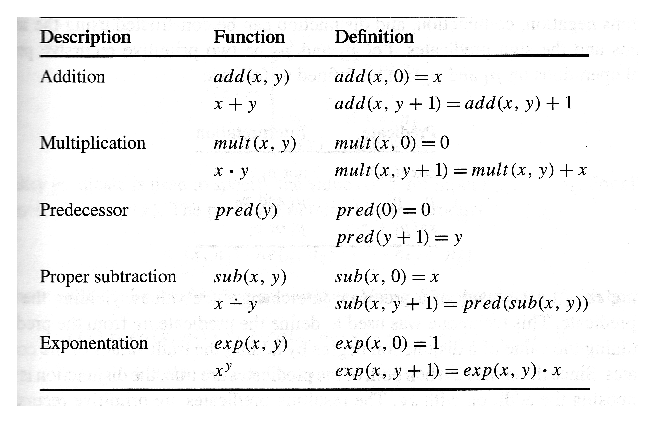
\includegraphics[height=60mm]{images/prfunctions.eps}
\end{center}

\es

\bs{Primitive Recursive Predicates}
{\small
We define primitive recursive predicates as primitive recursive functions with
the co-domain $\{0,1\}$.

\begin{center}
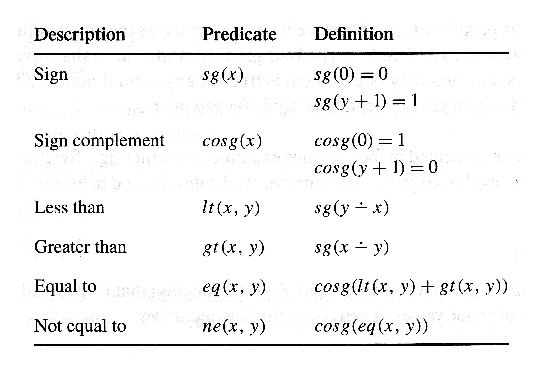
\includegraphics[height=60mm]{images/prpredicates.eps}
\end{center}
}


\es


\bs{Primitive Recursive Functions}
\small
{\bf Theorem:} Let $g(x)$ be a primitive recursive function, then the function
\[
f(x) = \left \{
	\begin{array}{ll}
	y_1 & \text{if $x = n_1$}\\
	y_2 & \text{if $x = n_2$}\\
	\vdots&\vdots\\
	y_k & \text{if $x = n_k$}\\
	g(x) & \text{otherwise}
	\end{array}
	\right .
\]
is also primitive recursive.

{\bf Proof:} We can express $f(x)$ as the following function using the primitive recursive 
predicates $eq$ and $ne$, multiplication, and addition,
\[
f(x) = eq(x,n1)\cdot y_1 + \ldots +eq(x,n_k)\cdot y_k + ne(x,n_1)\cdot\ldots\cdot ne(x,n_k)\cdot g(x)
\]
\es

\bs{Primitive Recursive Functions}
\small
{\bf Theorem:} Let $g(x,y)$ and $h(x)$ be primitive recursive, then the functions,
\begin{enumerate}
\item $f(x,y,z_1,\dots,z_n) = g(x,y)$
\item $f(x,y) = g(y,x)$
\item $f(x) = g(x,x)$
\item $f(x) = h(0)$
\end{enumerate}
are also primitive recursive.

{\bf Proof:}  We show primitive recursion by construction,
\begin{enumerate}
\item $f = g \circ (p^{(n+2)}_1, p^{(n+2)}_2)$
\item $f = g \circ (p^{(2)}_1, p^{(2)}_2)$
\item $f = g \circ (p^{(1)}_1, p^{(1)}_1)$
\item $f = h \circ z$
\end{enumerate}
\es


\bs{Bounded Minimalization}
\small
Bounded minimalization is defined via the search operator $\mu^y$,
\[
f(x_1,\ldots,x_n,y) = \mu^y z[p(x_1,\ldots,x_n,z)],
\]
and defines a function $f$ which reads ``return the least value of $z$ satisfying $p(x_1,\ldots,x_n,z)$
or return the bound,'' more precisely 
\[
f(x_1,\ldots,x_n,y) = \left \{
	\begin{array}{ll}
	\min z &\text{s. t. $p(x_1,\ldots,x_n,z) = 1$ and $0 \le z \le y$}\\
	y + 1 &\text{otherwise}
	\end{array}
	\right .
\]
The $\mu$ operator can be viewed as a search operator over the natural numbers $\le y$
for the minimal value that satisfies the predicate $p$.  
Consider,
\[
f(x,y) = \mu^y z[eq(x, mult(z,z)].
\]
Here $f(4,10) = 2$ and $f(3,10)= 11$.

{\bf Theorem:} Let $p(x_1,\ldots,x_n,z)$ be a primitive recursive predicate, then the function
\[
f(x_1,\ldots,x_n,y) = \mu^y z[p(x_1,\ldots,x_n,z)],
\]
is also primitive recursive.

{\bf Proof:} On can construct the bounded minimalization of bounded sum.  See proof on handout,
Theorem 13.3.3.
\es



\bs{Primitive Recursive Functions}

\fframe{{\bf Theorem:} Every primitive recursive function is computable.}

{\bf Proof Sketch:} It is clear that the zero, successor, and projection functions are
computable by their sheer simplicity.  It remains to show that computable functions
are closed under composition and recursion. This can be shown by constructing 
the appropriate TMs.

(Start by constructing TMs for the basis functions and then plug these simple machines together
to obtain more complex ones.  Idea: universal turing machines that executes encodings of
machines.)
\es


\bs{General Recursive Functions}
\small
\fframe{{\bf Theorem:} There exist total computable functions not representable by primitive recursion.}

{\bf Proof:} By counter example. We can prove this by construction, e.g., Ackermann's function,
\[
A(m,n) = \left \{
\begin{array}{ll}
n + 1 & \text{if $m = 0$}\\
A(m-1,1) &\text{if $m>0$ and $n = 0$}\\
A(m-1,A(m,n-1)) &\text{if $m>0$ and $n>0$},
\end{array}
\right .
\]
where $m,n \ge 0$.

This is a recursive function, but it is not primitive recursive: you cannot define this function
according to the primitive recursive function template.
\es


\bs{Partial Functions}

\vspace{.2in}
We relax our notion of computable functions by defining the notion of partial
computable function as a Turing machine that does not halt for some of the inputs
of the function it implements.  In effect the function will then be undefined for 
these input values, as required by the mathematical definition of partial function.
\es

\bs{Unbounded Minimalization}
{\small
The consequence of the previous arguments is that in order for recursion to provide
a computational framework equivalent to Turing machines we will need
to {\em admit partial functions}.

We do so by introducing the {\bf\em unbounded minimalization operator} $\mu$,
\[
f(x_1,\ldots,x_n) = \mu z[p(x_1,\ldots,x_n,z)],
\]
defines a function $f$ which reads ``return the least value of $z$ satisfying $p(x_1,\ldots,x_n,z)$,'' or 
\[
f(x_1,\ldots,x_n) = \min z, \hspace{.2in}\mbox{s. t. $p(x_1,\ldots,x_n,z) = 1$}.
\]
The $\mu$ operator can be viewed as a search operator over the natural numbers
for the minimal value that satisfies the predicate $p$.  That $f$ represents a partial 
function comes from the fact that perhaps no such natural number exists and the
search will go on forever. Consider,
\[
f(x) = \mu z[eq(x, mult(z,z)].
\]
Here, $f(3)\uparrow$.
}
\es

\bs{$\mu$-Recursive Functions}

\begin{center}
\includegraphics[height=40mm]{images/mu-rec-functions.eps}
\end{center}
\es

\bs{$\mu$-Recursive Functions}

\fframe{{\bf Theorem:} Turing machines and  $\mu$-recursive functions are equivalent.}

{\bf Proof Sketch:} By construction.

(a) We first show that Turing machines can simulate $\mu$-recursive functions.  We have already shown that TMs can implement
the primitive recursive functions.  Since composition is strict it suffices to show that a Turing machine implementation
of the $\mu$ operator exists for the ``if'' direction.  Since this is a search procedure it
is clear that it is algorithmic and a machine can be built for that.

(b) For the converse we provide a procedure to encode any TM as a function based on
an enumeration of all possible configurations.  Since the enumerations are countable (think of them as binary encoded, finite strings), this is possible and therefore it is possible to construct a function representing a TM.

\es

\bs{\large $\lambda$-Calc Implementation}

\fframe{{\bf Theorem:} If a function is computable by a $\lambda$-expression then it is computable by a Turing machine.}

{\bf Proof Sketch:} By construction.  Computing with $\lambda$-expressions is algorithmic.  It is straightforward
to construct an encoding for $\lambda$-expressions and then perform the algorithm for function applications.
That this is possible is demonstrated that we have functional programming languages running on Von Newmann
style computers.

\es

\bs{\large $\lambda$-Calc Implementation}

\fframe{{\bf Theorem:} $\mu$-recursive functions can be implemented in the $\lambda$-calculus.}

{\bf Proof Sketch:} Since they are functions and the $\mu$ operator is algorithmic it is clear that the functions
can be implemented in the $\lambda$-calculus.  Consider,
\begin{itemize}
\item The zero, successor, and projection functions,
\begin{eqnarray*}
\mbox{ZERO} &=& \lambda x.\, 0\\
\mbox{SUCC} &=& \lambda x.\, x+1\\
\mbox{PROJ}_i^n &=& \lambda(x_1,\ldots,x_n).\, x_i
\end{eqnarray*}

\item The composition of the function $h$ with the functions $g_1, g_2,\dots, g_n$, applied to the tuple $(x_1,x_2,\ldots,x_k)$ is $h(g_1(x_1,x_2,\ldots,x_k),g_2(x_1,x_2,\ldots,x_k),\ldots,g_n(x_1,x_2,\dots,x_k))$,
or as a $\lambda$-expression:
\[
\lambda f g_1\ldots g_n (x_1,x_2,\ldots,x_k).\,f \,(g_1(x_1,x_2,\ldots,x_k))\ldots(g_n(x_1,x_2,\ldots,x_k))
\]


\end{itemize}
\es

\bs{\large $\lambda$-Calc Implementation}

\begin{itemize}
\item The primitive recursive function $f$ with
\begin{eqnarray*}
f(x_1,\ldots,x_n,0) &=& h(x_1,\ldots,x_n)\\
f(x_1,\ldots,x_n,y)& = &g(x_1,\ldots,x_n,y-1,f(x_1,\ldots,x_n,y-1))
\end{eqnarray*}
can be written as the $\lambda$-expression
\[
\begin{array}{l}
\lambda h g .\,Y \, (\lambda f (x_1,\ldots,x_n) y. \\
\mbox{\hspace{.1in}}y = 0? \, (h\, (x_1,\ldots,x_n)) : (g\, (x_1,\ldots,x_n) \, (y - 1) \, (f \, (x_1,\ldots,x_n)\,(y-1))))
\end{array}
\]
Where $Y$ is called the fixed-point operator (or Y combinator) and is defined as
\[
Y = \lambda f.\, (\lambda x.\, f\, (x \,x)) (\lambda x.\, f\, (x\, x))
\]
This operator expresses recursive computation in pure $\lambda$-calculus.
\end{itemize}
\es

\bs{\large $\lambda$-Calc Implementation}

\begin{itemize}
\item The expression $\mu z[p(x_1,\ldots,x_n,z)]$ returns the smallest $z$ such that $p(x_1,\ldots,x_n,z)=0$, as a $\lambda$-expression:
\[
\lambda p\, (x_1,\ldots,x_n).\, (Y \,(\lambda h z.\, (p\, (x_1,\ldots, x_n)\, z) = 0? \, z : (h\, (z+1)))\, 0)
\]
\end{itemize}
This completes the proof. $\Box$
\es

\bs{The Equivalence}
\fframe{$\lambda$-Calculus $\prec$ Turing Machines $\prec$ $\mu$-Recursive Functions $\prec$ $\lambda$-Calculus}

where $a \prec b$ means $b$ implements $a$.
\es

\end{document}
%%%%%%%%%%%%%%%%%%%%%%%%%%% end of template1.tex %%%%%%%%%%%%%%%%%%%%%%%%%%%%%%%%

